\documentclass[UTF8]{article}

\usepackage{amsmath}
\usepackage{enumerate}
\usepackage{fancyhdr}
\usepackage{geometry}
\usepackage{graphicx}
\geometry{top=3cm,bottom=2.5cm,left=2.5cm,right=2.5cm}

\pagestyle{fancy}
\fancyhead[LO]{Ruiji Wei}
\fancyhead[RO]{Report}
\fancyhead[LE]{Ruiji Wei}
\fancyhead[RE]{Report}

\begin{document}
\begin{center}
    \section*{\textbf{Project Report}}
\end{center}

\section{Introduction}
\subsection{Introduction}
The project aims on finding an effective
and practical method to predict the revenue of a movie which is going to
be released in the future.
\subsection{Motivation}
As we can see and feel that movies play more and more important
role in our society. Many people enjoy watching moive during spare time with friends or family.
This is a great market for film company to make a profit. But not all films can gain great profit.
Some films can get reputation and high revenue at the same time but others may get a great loss.
So it is important for company to make a decision if they should shoot one film or not.
\subsection{Problem Definition}
The formal definition of this problem is that using old data records
to predict revenue of new released movie. It is a regression task.


\section{Prior Work}
\begin{itemize}
    \item Salzberg, Steven L. "C4. 5: Programs for machine learning by j. ross quinlan. morgan kaufmann publishers, inc., 1993." (1994): 235-240.
          Decision tree has been used in this project.
    \item Mansour, Yishay. "Pessimistic decision tree pruning based on tree size." MACHINE LEARNING-INTERNATIONAL WORKSHOP THEN CONFERENCE-. MORGAN KAUFMANN PUBLISHERS, INC., 1997.
          Decision tree pruning has been used to avoid overfitting problem
          because this method reduces the size of decision trees by removing sections of the tree that promises the tree does not memory all the information.
    \item Srivastava, Nitish, et al. "Dropout: a simple way to prevent neural networks from overfitting." The journal of machine learning research 15.1 (2014): 1929-1958.
          It was been planed to use dropout layer to solve overfitting problem of multilayer perceptron method.
\end{itemize}

\section{Model and Algorithm}
\subsection{Regression Tree}
Decision trees where the target variable can take continuous values
(typically real numbers) are called regression trees.

\subsection{Multilayer Perceptron}
In this project, I tried to use a simple multilayer perceptron model. For detail, I use
one layer with 100 hidden nodes, relu activation function and adam algorithm to do optimization.

\subsection{Similarity based method}
For this method, I use cosine similarity to measure similarity of two movies.
Prediction is based on similarity and movie budget(the reason will be explained in result and finding section).

\section{Results and Findings}
\subsection{Statistic Analysis}
\begin{itemize}
    \item The movies dataset has 4803 entries with 20 features: budget,genres...
          and credits dataset has 4083 entries with 4 features: movie\_id,title,cast and crew.
          These two dataset are merged into one pandans Dataframe.
    \item Do preprocessing for the whole data: removing duplicate data, add missing data and removing error data.
    \item Do subset selection. We should not use movies which have a low vote\_count because
          this means the vote is not trustable and could become noise of our dataset.
    \item Analyze revenue between some factors
          \begin{itemize}
              \item budget and revenue: From 2000 to 2015, budget of movies has not chanage a lot, but the revenue has increase on an even keel.
                    \begin{center}
                        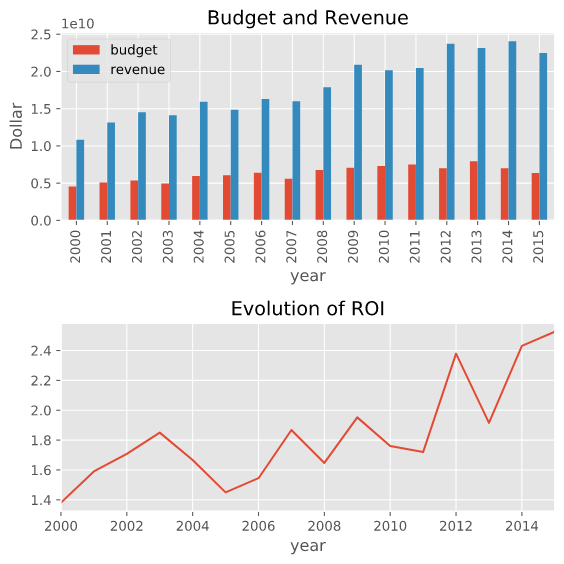
\includegraphics[scale=0.5]{Img/budget.png}
                    \end{center}
              \item rating and revenue: Generally, high rating means high revenue.
                    \begin{center}
                        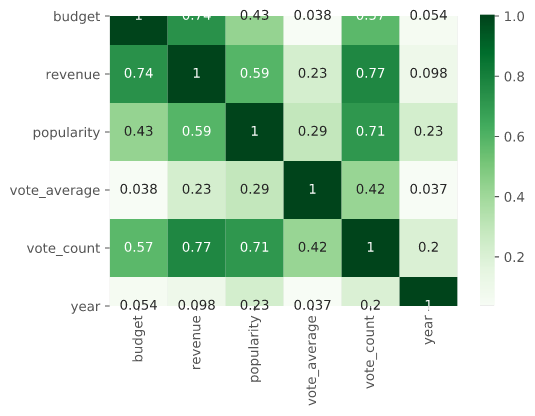
\includegraphics[scale=0.5]{Img/rating.png}
                    \end{center}
              \item genres and revenue: Top 5 high revenue genres is Animation, Fantasy, Adventure, Science Fiction and Action.
                    Movies of documentary has the highest return rate.
                    \begin{center}
                        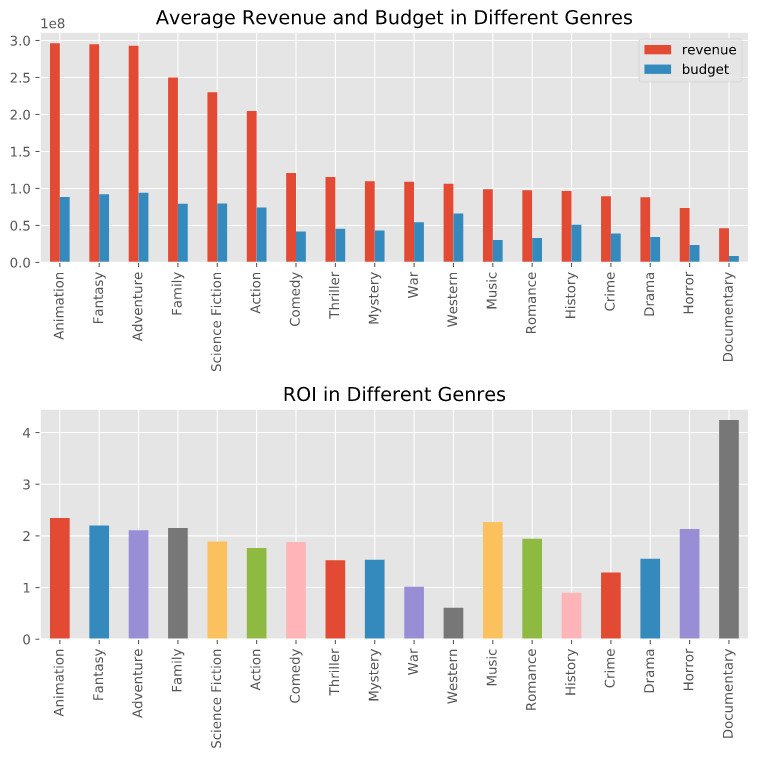
\includegraphics[scale=0.5]{Img/genres.png}
                    \end{center}
              \item director and revenue: James Cameron is the best director who is ahead of anyone else.
                    \begin{center}
                        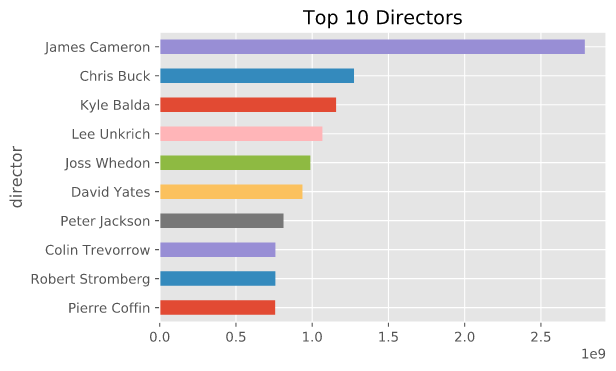
\includegraphics[scale=0.5]{Img/director.png}
                    \end{center}
              \item actor stars and revenue:
                    \begin{center}
                        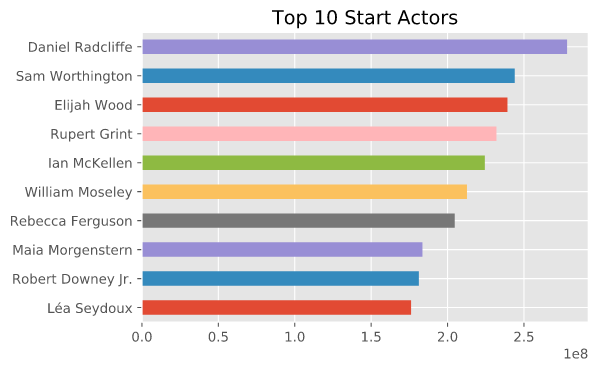
\includegraphics[scale=0.5]{Img/stars.png}
                    \end{center}
              \item released date and revenue: Movies which are released in May has the highest average revenue.
                    \begin{center}
                        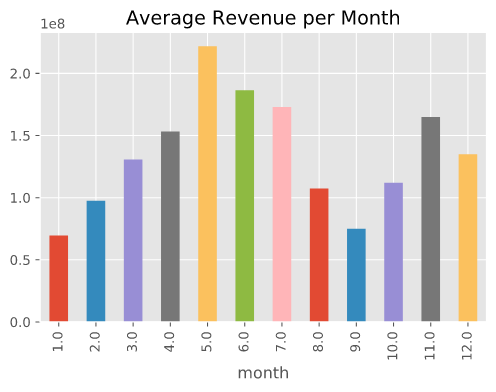
\includegraphics[scale=0.5]{Img/date.png}
                    \end{center}
          \end{itemize}
\end{itemize}


\subsection{Decision Tree Regression Method}
For the first time, the pruning technique has not been used and I got results that
accuracy on train dataset is 0.993 and on test dataset 0.057. Obviously, accuracy of train is
much higher than test and the decision tree picture shows a very high depth and large leaf nodes.
Therefore, we can infer the tree overfits data of train datasets. In this case,
the tree may just memorys all the data instead of learning knowladge of data.
So I tried to limit the max depth (set the max\_depth argument equals to 5) of tree
to overcome the overfitting problem. But unfortunately, accuracy both on train and test
reduced to an unacceptable value. There are 0.098 and 0.093. Eventhough the two accuracy is closer than
before we can not use this method because such low accuracy makes no sense.
\subsection{Multilayer Perceptron}
For this method, the argument sets are as following: 1 hidden layer with 100 nodes, relu activation function
adam optimization method, constant learning rate 0.001, iteration times 1000.\\
The result is not satisfactory. The accuracy on train and test are 0.080 and 0.093.
My analysis is that there exists an awkward situation. Our dataset has features with different type.
Three of them are categorical data and the budget feature is in numerical type and it is much larger than
others. For general case, we can do normalize to eliminate this kind of problem.
But it is not explicable to do this for categorical variable. Therefore, the budge feature
takes dominate the prediction value means the model may not take full adbantage of all data feature.
That is why it performs not good.
\subsection{Similarity Based Method}
Inspired by the method and principle of collaborative filtering, I tried to predict revenue of new movie
by comparing the similarity between new movie and recorded data. The method have three main steps:
1. calculate the similarity of new movie between others, select the top 5 similair movies. \\
2. calculate the average budget and revenue ratio of the five films.\\
3. use this return rate to predict the income of the new movie.\\
There is one thing I need to emphasize. I don not just measure similarity and use average revenue
as the prediction. I have tried this kind of method but the result is not good. But we can see from
previous statistic analysis that the return rate of movie is relatively stable. According to this finding,
the prediction should be influenced by budget greatly and the other features play a regulating role.
Finally, the model got an satisfactory outcome. I used the k-fold cross validation to evaluate the model.
The result are as follows(k=3):
\begin{center}
    \begin{tabular}{|c|c|c|}
        \hline
        Iteration & Accuracy of Train & Accuracy of Test \\
        \hline
        1         & 0.943             & 0.943            \\
        \hline
        2         & 0.935             & 0.927            \\
        \hline
        3         & 0.918             & 0.934            \\
        \hline
        Average   & 0.932             & 0.934            \\
        \hline
    \end{tabular}
\end{center}

\end{document}